\section{Signale und Systeme}
	\begin{tabular}{|l|l|}
    	\hline
    	\textbf{Linearität} & \textbf{Zeitinvarianz}\\
    	\hline
    	$S(x1+x2)=S(x1)+S(x2)$ & $S(x(t-t_0)=S(x)\cdot x(t-t_0)$ \\
    	$S(c\cdot x)=c\cdot S(x)$ & \\
		\hline    
    \end{tabular}
	
	\subsection{Lineare zeitinvariante Systeme (LTI-Systeme)}
		LTI-Systeme sind durch ihre Impulsantwort $h$ vollständig bestimmt\\ \\	
		\textbf{Berechnung der Systemantwort von kontinuierlichen LTI-Systemen}\\
		\begin{tabular}{ll}
			\parbox{8cm}{
			$$s_2(t) = h(t) * s_1(t) \laplace S_2(s) = H(s) S_1(s)$$
			$$h(t) \laplace H(s)$$}
			& \parbox{4cm}{
			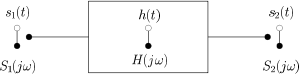
\includegraphics[width=5cm]{./bilder/utf-theorie.png}}\\
		\end{tabular} \\
		Amplitudengang: 		$|H(\omega)| = \begin{cases}
								< 1 \text{ Dämpfung} \\
								> 1 \text{ Verstärkung}
								\end{cases}$	\\
		\textbf{Sprungantwort} \\
		Die Sprungantwort $y_{\sigma}(t)$ ist die Systemantwort auf die
		Sprungfunktion $\sigma(t)$: \\ $Y_{\sigma}(s)=H(s) \cdot \Sigma(\omega)$

	\subsection{Eigenfrequenz, Frequenzgang}
	Zu jeder Frequenz gehört der eigene Frequenzgang mit $a, b \in \mathbb{C}$\\
	$$a e^{j\omega_1 t} + b e^{j\omega_2 t} \rightarrow a H(\omega_1) e^{j\omega_1 t} + b H(\omega_2) e^{j\omega_2 t}$$
	Frequenzgang bei Spektraldarstellung: $$\sum_{k=-\infty}^{\infty} c_k e^{jk\omega t} \rightarrow \boxed{H(\omega)}
	\rightarrow \sum_{k=-\infty}^{\infty} c_k H(\omega k) e^{jk\omega t}$$			
		
	\subsection{Faltung}
	\begin{tabular}{|l|} \hline
	$y(t) = f(t)\ast g(t) = g(t) \ast f(t) = (f \ast g)(t) :=
	\int\limits_{-\infty}^\infty f(u) \cdot g(t-u)\,du =
	\int\limits_{-\infty}^\infty f(t-u) \cdot h(u)\,du $ \\ \hline
	\end{tabular} \\
	
	Hat $g\left(t\right)$ keine negative Argumente dann gilt :
	$\left(g \ast f \right)\left(t\right)=\int\limits_{-\infty}^t f(u) \cdot
	g(t-u)\,du$\\
	Hat $f\left(t\right)$ keine negative Argumente (Einschaltvorgang) dann gilt :
	$\left(g \ast f \right)\left(t\right)=\int\limits_{0}^t f(u) \cdot
	g(t-u)\,du$\\
	Bei einer Faltung mit einer $\delta\left(t\right)$Funktion
	gilt:$f\left(t\right) \ast \delta\left(t\right) = f\left(t\right)$\\
	
	\textbf{Grafische Interpretation:}
	Einfacheres Signal an der Y-Achse spiegeln, um t nach rechts verschieben, Signale
	multiplizieren und integrieren. \\
	\textbf{Bestimmung der Grenzen:}
	Koordinatensystem mit t auf X-Achse und u auf Y-Achse. Einzeichnen, in welchen Bereichen
	die Faktoren $0$ werden. Integriert werden muss nur, wo Signal $\neq 0$ ist. 
